\documentclass[a4paper, 11pt]{scrreprt}

\usepackage{ngerman}
\usepackage{float}
\restylefloat{figure}
\usepackage{graphicx}
\parindent0pt

\usepackage{chngcntr}
\counterwithout{table}{chapter}
\counterwithout{figure}{chapter}

\usepackage{tocloft}
\renewcommand{\figurename}{Abbildung}
\renewcommand{\tablename}{Tabelle}
\renewcommand{\cftfigpresnum}{Abb. }
\renewcommand{\cfttabpresnum}{Tab. }

\renewcommand{\cftfigaftersnum}{:}
\renewcommand{\cfttabaftersnum}{:}

\setlength{\cftfignumwidth}{2cm}
\setlength{\cfttabnumwidth}{2cm}

\setlength{\cftfigindent}{0cm}
\setlength{\cfttabindent}{0cm}

\usepackage[margin=25mm,right=25mm, left=25mm]{geometry}


\author{Timo Schwertfeger, Daniel Kaiser, Patrick Preu"s}



\title{Dokumentation f"ur das Softwaretechnik-Projekt AppCiMo (application for city movement)
\newline
\newline
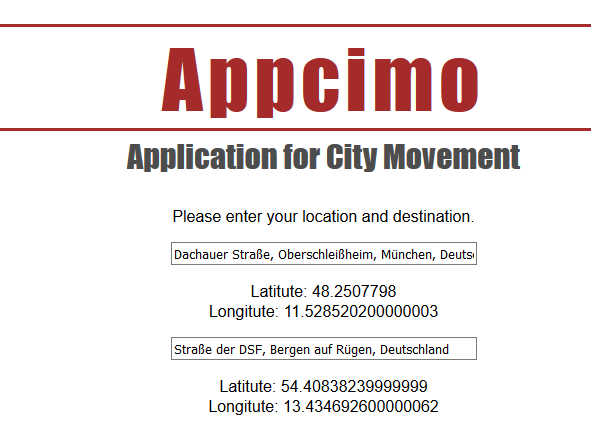
\includegraphics[width=0.7\textwidth]{appcimo.png}}



\begin{document}

\maketitle

\setcounter{secnumdepth}{5}
\setcounter{tocdepth}{5}

\tableofcontents


\chapter{Einleitung}





\section{Ausgangssituation}
In deutschen Gro"sst"adten gibt es eine Vielzahl von M"oglichkeiten schnell von A nach B zu kommen. Dies ist vor allem der au"serordentlichen Verkehrsinfrastruktur zu verdanken. Jedem B"urger ist die Wahl selbst "uberlassen, ob er mittels eines Privat-PKW’s, mit den "offentlichen Verkehrsmitteln oder zum Beispiel mit dem Fahrrad seinen Bestimmungsort erreichen m"ochte. Doch in Gro"sst"adten, wie zum Beispiel Berlin, kann dieses "Uberangebot an Transportm"oglichkeiten oft auf Situationen sto"sen, in denen sich der/die Zielsuchende nicht sicher ist, welche Transportm"oglichkeit die beste f"ur ihn oder sie ist. Hier spielen Faktoren wie die innerst"adtische Verkehrssituation, Verf"ugbarkeit von Car-Sharing Autos in der N"ahe, Stra"sensperrungen oder Preise f"ur die "offentlichen Verkehrsmittel eine Rolle. All diese M"oglichkeiten abzuw"agen, um m"oglichst schnell und g"unstig einen Zielort zu erreichen kann unter Umst"anden ein zu gro"ser Aufwand sein. \\

Das Team AppCiMo m"ochte gerne etwas Licht in diesen Gro"sstadtdschungel bringen und verschiedene M"oglichkeiten f"ur den eigenen Personentransport in (Gro"s-)St"adten "ubersichtlich und ansprechend aufzeigen.



\section{Zielsetzung}
Ziel des Projektes ist die Planung und Entwicklung eines City-Movement-Prototypen in Form einer One-Page Webapplikation. Diese Webapplikation soll Nutzern als Entscheidungshilfe f"ur ihre Weg-Zielerreichung in deutschen Gro"sst"adten dienen. \\

Den Nutzern sollen ausgehend von Start- und Bestimmungsort, drei unterschiedliche Transportm"oglichkeiten f"ur ihre Zielerreichung aufgezeigt werden. Diese M"oglichkeiten umfassen Carsharing-Angebote in der N"ahe, "offentliche Verkehrsmittel und das eigene Fahrrad. Zus"atzlich sollen f"ur eine sofortige Einsch"atzung der ermittelten Transportm"oglichkeiten jeweils die Distanz, die voraussichtlich ben"otigte Zeit und die Kosten dargestellt werden. \\

\textbf{Features:}
\begin{itemize}
\item Mindestens drei verschiedene Transportm"oglichkeiten um das Ziel zu erreichen\\
\item Kurzansichten und detaillierte Ansichten\\
\item Preisermittlung f"ur jede Transportm"oglichkeit\\
\item Kartenvorschau in GoogleMaps\\
\item Wegbeschreibung zu dem Ziel\\


\end{itemize}

Bei Appcimo handelt es sich um eine browserbasierte Webapplikation, d.h. f"ur die Nutzung ist eine Internetverbindung notwendig. Au"serdem ist eine automatische Standorterfassung von Vorteil.
Diese Webapplikation soll auf den g"angigen Browsern stabil laufen.


\chapter{Projektvorbereitung}
F"ur die Planung, Organisation, Aufteilung und Verfolgung des Projekts wird die Projekt Management Plattform \textbf{Taiga.io} verwendet. Taiga.io ist ein webbasiertes open-source Projekt-Management-Tool f"ur agile Entwickler, Designer und Projektmanager. Die St"arken liegen vor allem in den individuellen Anpassungsm"oglichkeiten, sowie in der einfachen und intuitiven Bedienung. Es wird von Start-Ups bevorzugt verwendet.


\section{Projektmanagementsoftware Taiga.io}

\subsection{Vorgehensmodell}
Das Projekt Appcimo wird anhand des Scrum Vorgehensmodells bearbeitet.

\begin{figure} [H]
\begin{center}


\includegraphics[width=12cm]{Scrum.png}
\caption{Scrum Infografik}
\label{Scrum_logo}

\end{center}
\end{figure}

Dabei werden vor allem folgende Vorz"uge von Scrum in dem Projekt genutzt:

\begin{itemize}
\item{wenige, leicht verst"andliche Regeln}
\item{Kurze Kommunikationswege}
\item{Hohe Flexibilit"at/Agilit"at durch adaptives Planen}
\item{Hohe Effektivit"at durch Selbstorganisation}
\item{Hohe Transparenz durch regelm"a"sige Meetings und Backlogs}
\item{Zeitnahe Realisation neuer Produkteigenschaften bzw. Inkremente}
\item{Kontinuierlicher Verbesserungsprozess}
\item{Kurzfristige Problem-Identifikation}
\item{Geringer Administrations- und Dokumentationsaufwand}
\end{itemize}


\textbf{Die Scrum-Rollen}

Die Umst"ande in denen die Webapplikation Appcimo entwickelt wird, f"uhren im Projektteam zu einer abgewandelten Form der klassischen Scrum-Vorgehensweise. \\

Somit gibt es im Projektteam keine festen Rollen wie Product Owner, Entwickler und Scrum Master. Jedes Projektmitglied ist Product owner und Scrum master. Pers"onliche Pr"aferenzen lassen jedoch eine Spezialisierung wie Entwicklung, Dokumentation oder das Schaffen von wichtigen Voraussetzungen zu. Das Ziel ist hier eine ausbalancierte und effiziente Projektumgebung zu schaffen, in dem jedes Projektmitglied seine St"arken ausspielen kann und seine W"unsche ber"ucksichtigt werden. \\


\textbf{Die Scrum-Artefakte} \\

Product Backlog: Darin sind die Anforderungen an die Webapplikation in Form eines vorl"aufigen Plans erfasst - dieser ist dynamisch und wird kontinuierlich weiterentwickelt. \\

Sprint Backlog: Basierend auf dem Product Backlog werden hier die im jeweiligen Sprint zu erledigenden Aufgaben f"ur alle Projektbeteiligten einsehbar hinterlegt.\\

Product Increment: Das Produkt-Inkrement ist das erledigte Arbeitspaket, welches nach Ende eines Sprints als fertiges Teilprodukt geliefert wird.\\



\textbf{Die Scrum-Aktivit"aten}\\

Sprint Planning: F"ur jeden Sprint muss geplant werden, welches neue Feature w"ahrend eines Sprints realisiert werden kann.\\

Daily Scrum: Der ‘Daily Scrum‘ wird in einer abgewandelten Variante in Form eines ‘Weekly Scrum’ realisiert. Das Ziel hier ist prim"ar der Austausch untereinander im Projektteam bzgl. Probleme, Ideen, L"osungen und Entscheidungen.\\

Sprint Review: Eine nachtr"agliche Bewertung der zu umsetzenden Features, ob  das im Sprint Backlog formulierte Entwicklungsziel aus Sicht des Projektteams zu 100 Prozent erreicht wurde.\\

Sprint-Retrospektive: Ein Kontrollmechanismus, ob die bisherige Arbeitsweise verbessert werden kann.\\

Product Backlog Refinement: Im Projektteam wird untersucht, inwieweit der im Product Backlog erfasste Plan bzw. die Produkt-Vision auf Basis neuen Wissens verbessert werden kann.


\subsection{Auswahl Taiga.io}

F"ur das Projektmanagement ist es wichtig eine geeignete Projektmanagementsoftware zu finden, die sich an die Bed"urfnisse
des Softwareprojektes anpassen l"asst. Nach Recherchen und Austausch mit Kommolitonen und Arbeitskollegen wurde uns Taiga.io empfohlen. Taiga.io ist eine webbasierte Projektmanagement-Software, die eine Projektdurchf"uhrung mit Scrum
erm"oglicht. Integration von Github ist ebenso m"oglich, wie die Einrichtung von Plugins, z.B. Chat-Programmen, z.B HipChat oder Slack.

\subsection{Einrichtung des Projektteams}

Sobald die Registrierung in Taiga.io erfolgt ist, gelangt man auf das allgemeine Dashboard, wor"uber die Projekte verwalten werden und die aktuellen Informationen eingesehen werden k"onnen.\newline

\begin{figure} [H]
\begin{center}


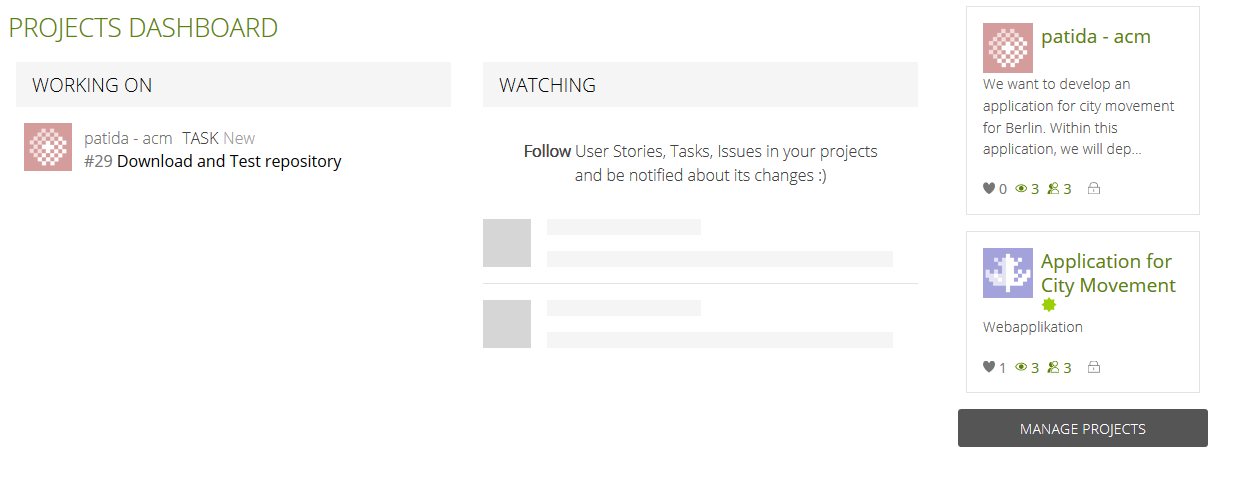
\includegraphics[width=16cm]{dashboard.png}
\caption{Taiga.io Dashboard}

\end{center}
\end{figure}

"Uber das Men"u "`MANAGE PROJECTS"' ist es m"oglich, bestehende Projekte zu verwalten und neue Projekte anzulegen. Zur kostenlosen Nutzung ist die Erstellung eines privaten Projekts mit maximal vier Usern m"oglich oder beliebig viele "offentliche Projekte. Sobald das Projekt erstellt ist, k"onnen im Admin-Men"u User hinzugef"ugt und die entsprechenden Rollen im Scrum-Vorgehensmodell zugewiesen werden.

\begin{figure} [H]
\begin{center}


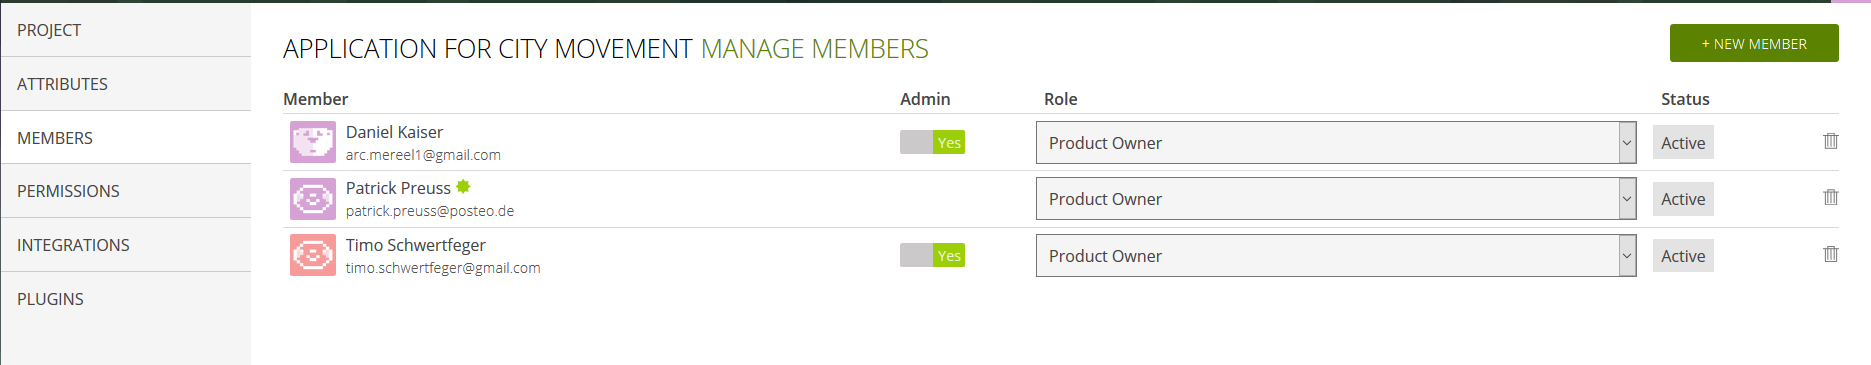
\includegraphics[width=16cm]{members.png}
\caption{Taiga.io Admin-Members}

\end{center}
\end{figure}

Wir haben uns entschieden, allen Projektbeteiligten die Rolle Product Owner zuzuweisen, da eine strikte Durchf"uhrung von Scrum in einem kleinen Team kaum m"oglich ist.

\subsection{Integration HipChat}

Um eine schnelle Kommunikation innerhalb des Projekts entschieden wir uns f"ur eine Chat-L"osung, die als Windows-Applikation und Smartphone-App verf"ugbar ist. F"ur die Durchf"uhrung des Projektes nutzten wir HipChat von Atlassian. Die Integration in Taiga.io funktioniert mit Hilfe eines Webhooks, der mit HipChat erzeugt wird und in Taiga.io integriert wird. Somit wird eine Benachrichtigung "uber s"amtliche Aktiviat"aten erm"oglicht.

\begin{figure} [H]
\begin{center}

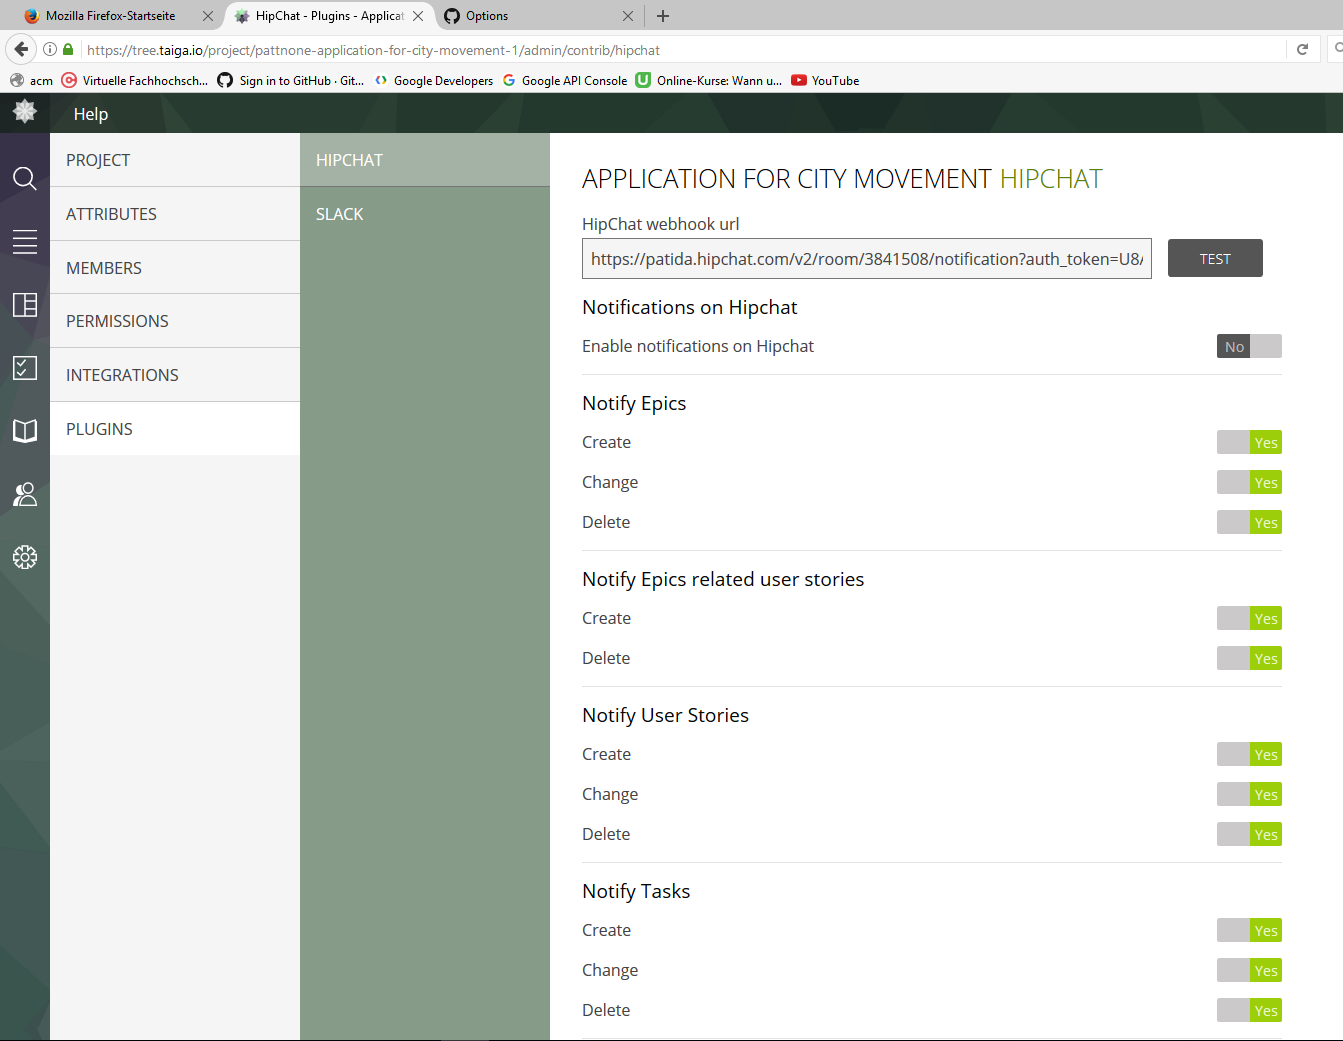
\includegraphics[width=16cm]{hipchat.png}
\caption{Taiga.io HipChat-Integration}

\end{center}
\end{figure}

Zus"atzlich integrierten wir Github in den HipChat, um "uber Commits und Pushes benachrichtigt zu werden.

\begin{figure} [H]
\begin{center}


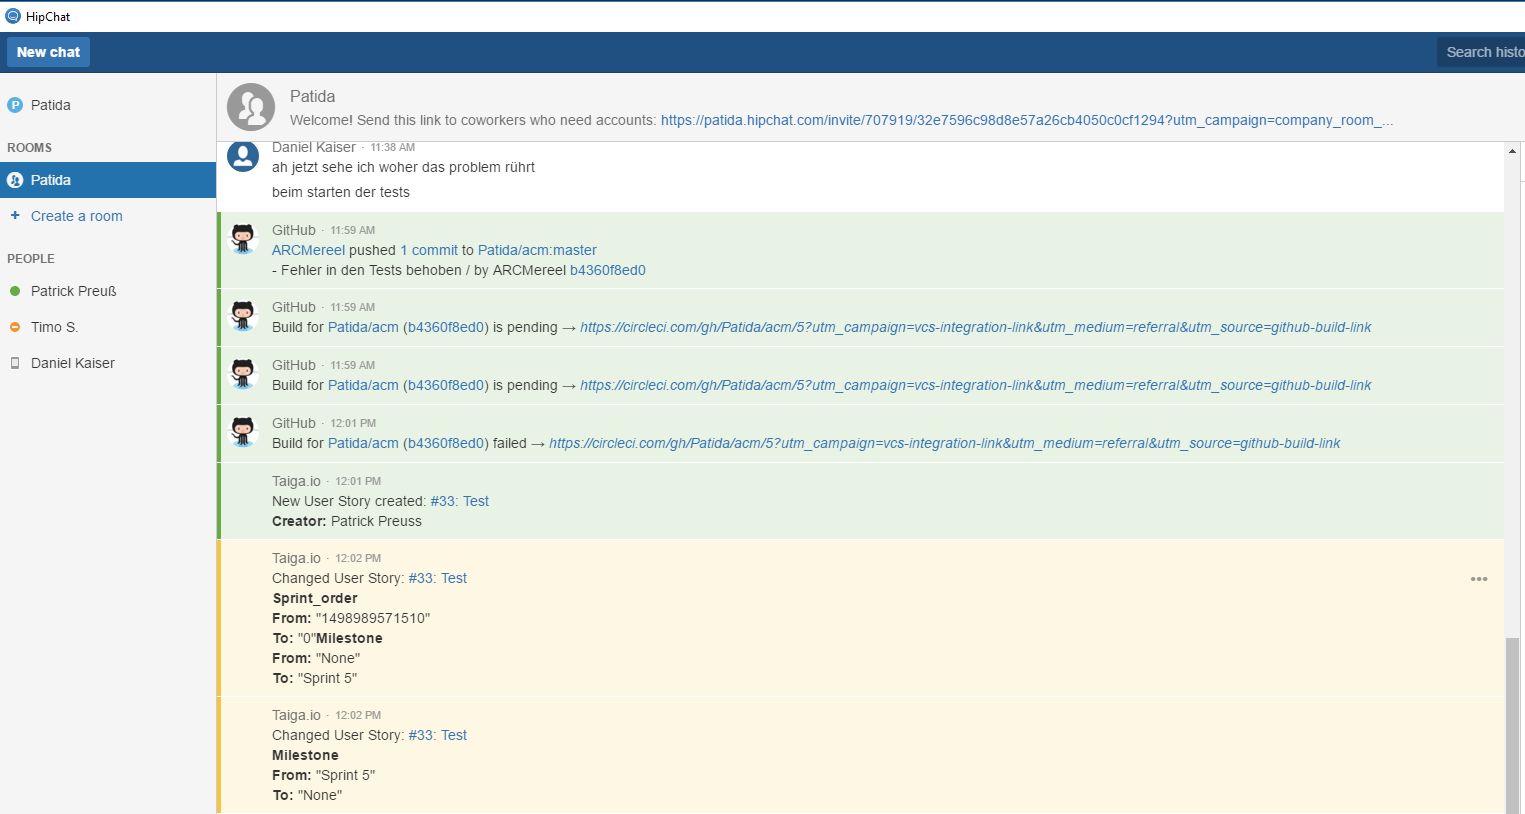
\includegraphics[width=16cm]{info_taiga_github_hipchat.png}
\caption{Taiga.io HipChat-Integration}

\end{center}
\end{figure}


\subsection{Definition von User-Stories}

User-Stories werden mit Taiga.io im Backlog "uber "`NEW USER STORY"' erstellt. Nachdem die User-Story erstellt ist, kann die User-Story einem geplanten Sprint zugeordnet werden.

\begin{figure} [H]
\begin{center}

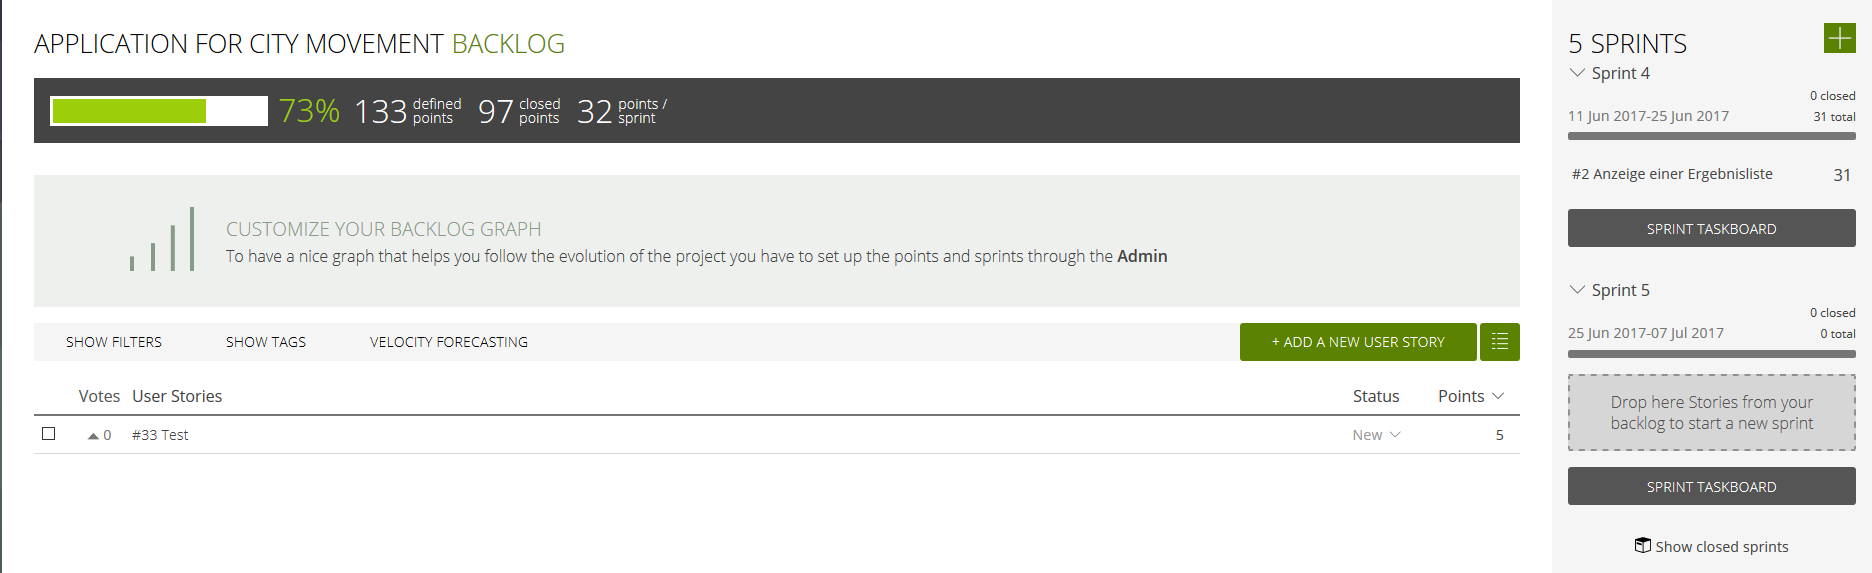
\includegraphics[width=16cm]{backlog.png}
\caption{Taiga.io Backlog}

\end{center}
\end{figure}

Die definierten User-Stories sind unter dem Punkt 3.4 aufgef"uhrt.


\subsection{Definition von Tasks}

Die Tasks zu den User-Story werden im Sprinttaskboard erstellt und k"onnen via Drag \& Drop den Spalten "`New"', "`In Progress"', "`Ready for Test"', "`Closed"' oder "`Need Information"' zugewiesen werden. Somit ist eine "Ubersicht des Sprint im Allgemeinen und des Fortschritt der Tasks ersichtlich.

\begin{figure} [H]
\begin{center}

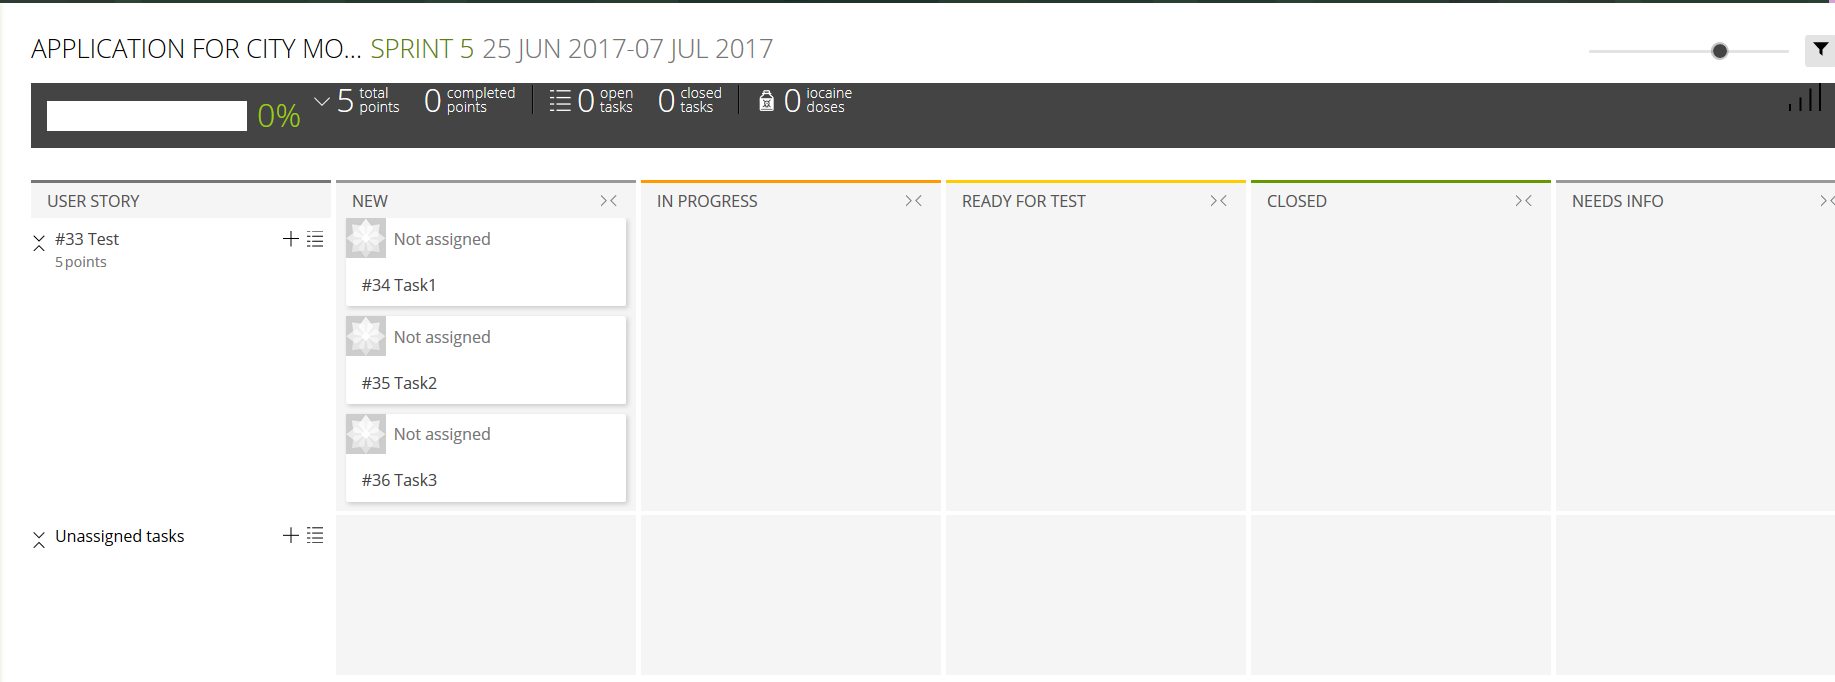
\includegraphics[width=16cm]{sprint_tasks.png}
\caption{Taiga.io Sprinttasks}

\end{center}
\end{figure}

\section{Projektdurchf"uhrung}

\subsection{Sprintplanung}

Zur Planung des Projektes haben wir sechs Sprint den Gesamtzeitraum des Projekts definiert. Jeder Sprint dauert zwei Wochen. Dadurch wird gew"ahrleistet, dass der Sprint mit allen Schritten der Iterationen durchgef"uhrt werden kann.

\begin{figure} [H]
\begin{center}

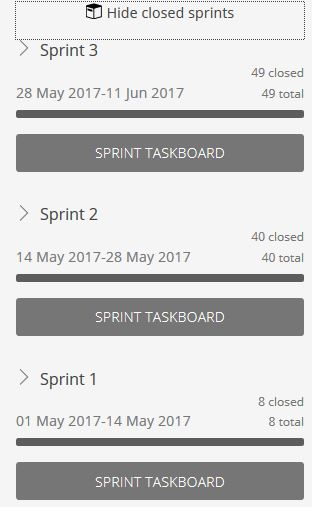
\includegraphics[width=6cm, height=10cm]{sprint_2.jpg}
\caption{Taiga.io Sprints 1-3}

\end{center}
\end{figure}

\begin{figure} [H]
\begin{center}

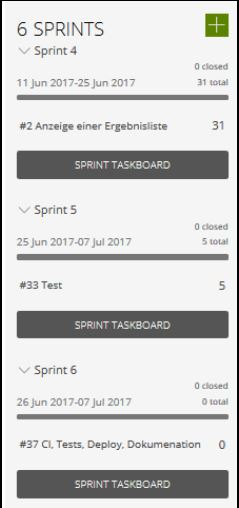
\includegraphics[width=6cm, height=10cm]{sprint_1.jpg}
\caption{Taiga.io Sprints 4-6}

\end{center}
\end{figure}

\subsection{Retrospektive}

Nach jedem Sprint tauschten wir uns
bez"uglich unser Ergebnisse aus.
Somit ergaben sich Verbesserungsvorschläge für das weitere Vorgehen,
sowie für die Planung weiterer Sprints.
Der Austausch ist wichtig, um Einsicht in die
Aufgaben jedes einzelnen Teammitgliedes zu erhalten. Die Retrospektive ist ein gutes Mittel, um alle Teammitglieder als Gruppe enger zusammen zu f"uhren. Konflikt innerhalb des Sprints wurden aufgezeigt, somit wurde Frust innerhalb des Teams vermieden.

\chapter{Produktanforderungen}

\section{Funktionale Anforderungen}

\begin{table}[H]

\caption{funktionale Anforderungen}

\ \\

\par

\label{tab:Tabelle1}

\centering

\begin{tabular}{|p{2.5cm} p{12cm}| ll}

\hline

Nr.	& Beschreibung\\

\hline

FU01 &	Das System muss f"ahig sein JSON-Objekte aus den Anfragen an die Google API zu verarbeiten.\\

\hline
FU02 &	Sobald der Benutzer eine Verbindung sucht, muss das System dem Benutzer die M"oglichkeit bieten einen Start- und Zielort einzugeben.\\

\hline
FU03& Sobald der Benutzer den Start- und Zielort eingibt, muss das System die M"oglichkeit bieten, dem Benutzer eine Vorschlagsliste w"ahrend der Eingabe anzuzeigen.\\

\hline
FU03.01	&Die Vorschlagsliste muss bei der Eingabe des ersten Zeichens angezeigt werden.\\

\hline
FU03.02	&Die vorgeschlagenen Tupel sollen mit folgender Reihenfolge angezeigt werden, 1. Stra"se, 2. Ort, 3. Postleitzahl\\

\hline
FU04	&Sobald der Benutzer Start und Zielort eigegeben hat, muss das System die M"oglichkeit bieten, die gesuchte Verbindung mit unterschiedlichen Transportmitteln anzuzeigen.\\

\hline
FU04.01	&Das Transportmittel „zu Fu"s“ muss ausw"ahlbar sein.\\

\hline
FU04.02&	Das Transportmittel  „Auto“ muss ausw"ahlbar sein.\\

\hline
FU04.03	&Das Transportmittel „"offentliche Verkehrsmittel“ muss ausw"ahlbar sein.\\

\hline
FU05	&Falls der Benutzer die Suchanfrage "andert, muss das System die M"oglichkeit bieten, die gesuchte Verbindung und die Karte zu aktualisieren.\\

\hline
FU05.01	&Die Vorschlagsliste muss bei Neueingabe des Start- und Zielorts angezeigt werden.\\

\hline
FU05.02	&Die Verbindungskarte muss mit neuem Start- und Zielort die gesuchte Verbindung anzeigen.\\

\hline
FU05.03	&Die Distanz der neuen Verbindung muss aktualisiert werden.\\

\hline
FU05.04&	Die Dauer der neuen Verbindung muss aktualisiert werden.\\

\hline
FU05.05	&Der Preis der neuen Verbindung muss angezeigt werden.\\

\hline
FU06	&Falls der Benutzer eine Verbindung sucht, muss das System die M"oglichkeit bieten, mehrere Transportmittel auszuw"ahlen.\\

\hline
FU07	&Sobald der Benutzer eine Verbindung sucht, muss das System die M"oglichkeit bieten, eine Ergebnisliste der gesuchten Verbindung anzuzeigen.\\

\hline
FU07.01&	In der Ergebnisliste muss der aktuelle Preis angezeigt werden.\\

\hline
FU07.02 &	In der Ergebnisliste muss die Dauer angezeigt werden.\\

\hline
FU07.03&	In der Ergebnisliste muss die Distanz angezeigt werden.\\

\hline


\end{tabular}

\end{table}

\section{Nicht-funktionale Anforderungen}

\begin{table}[H]

\caption{Projektanforderungen}

\ \\

\par

\label{tab:Tabelle2}

\centering

\begin{tabular}{|p{2.5cm} p{12cm}| ll}

\hline
Nr.	& Beschreibung\\

\hline
NFU01 &	Das System muss plattformunabh"angig und webbasiert sein. \\

\hline
NFU02 &	Das System muss mit einem Entwicklungs-Framework umgesetzt werden.\\

\hline
NFU03 &	Das System soll als Single-Page Anwendung umgesetzt werden.\\

\hline
NFU04 &	Das System soll gestestet werden.\\

\hline
NFU05 &	Das System soll "uber ein Deployment verf"ugen.\\

\hline
NFU06 &	F"ur Das System soll Continuous Integration konfiguriert werden.\\

\hline

\end{tabular}

\end{table}

\section{Projektanforderungen}

\begin{table}[H]

\caption{Nicht-funktionale Anforderungen}

\ \\

\par

\label{tab:Tabelle3}

\centering

\begin{tabular}{|p{2.5cm} p{12cm}| ll}

\hline
Nr. &	Beschreibung\\

\hline
PRJ01 &	F"ur die Umsetzung des Systems soll ein modernes Entwicklungs-Framework f"ur die Softwareerstellung genutzt werden.\\

\hline
PRJ02 &	Es muss eine Projektmanagementsoftware, f"ur die mit der Softwareerstellung einhergehende Projektarbeit, genutzt werden.\\

\hline
PRJ03 &	Der entwickelte Programmcode muss auf Github als Master-Branch hochgeladen werden.\\

\hline
PRJ04 &	F"ur das Software-Projekt muss eine Projektdokumentation erstellt werden.\\

\hline
\end{tabular}

\end{table}

\section{User-Stories und Sprint-Tasks}

\begin{table}[H]

\caption{Sprint 1}

\ \\

\par

\label{tab:Sprint 1}

\centering

\begin{tabular}{|p{2.5cm} p{12cm}| ll}

\hline
\multicolumn{2}{|l|}{US01 - Eingabe des Start- und Zielorts}  \\

\hline
Task \#7 & Felder erstellen f"ur die Eingabe eines Start- und Zielorts\\

\hline
\multicolumn{2}{l}{}\\

\hline
\multicolumn{2}{|l|}{US03 - Vorschlagsliste f"ur Eingabe des Start- und Zielorts}\\

\hline
Task \#8 & Einarbeitung in Google API Dokumentation f"ur Autocomplete-Funktion\\

\hline
Task \#9 & Autocomplete-Funktion in Felder des Start- und Zielorts implementieren\\

\hline

\end{tabular}

\end{table}

\begin{table}[H]

\caption{Sprint 2}

\ \\

\par

\label{tab:Sprint 2}

\centering

\begin{tabular}{|p{2.5cm} p{12cm}| ll}

\hline
\multicolumn{2}{|l|}{US06 - Auswahl verschiedener Transportmittel}\\

\hline
Task \#10 & Auswahl f"ur "offentliche Verkehrsmittel hinzuf"ugen\\

\hline
Task \#11 & Auswahl f"ur Car2Go/Auto hinzuf"ugen\\

\hline
Task \#12 & Auswahl f"ur Fahrrad hinzuf"ugen\\

\hline
Task \#31 & Mockup f"ur Car2Go Objekte erstellen und einbinden\\



\hline
\multicolumn{2}{l}{}\\

\hline
\multicolumn{2}{|l|}{US05 - Aktualisierung der Verbindungen nach "Anderung des Start- und/oder Zielorts}\\

\hline
Task \#13 & Aktualisierung der Google Karte bei "Anderungen implementieren\\

\hline
Task \#32 & Aktualisierung der Wegbeschreibung bei "Anderung implementieren\\

\hline

\end{tabular}

\end{table}

\begin{table}[H]

\caption{Sprint 3}

\ \\

\par

\label{tab:Sprint 3}

\centering

\begin{tabular}{|p{2.5cm} p{12cm}| ll}

\hline
\multicolumn{2}{|l|}{US04 - Anzeige von Verbindungen auf der Karte} \\

\hline
Task \#14 & Google map f"ur Autofahrt implementieren\\

\hline
Task \#15 & Google Map f"ur Fahrt mit "offentlichen Verkehrsmitteln implementieren\\

\hline
Task \#16 & Google Map f"ur Fahrradfahrt implementieren\\

\hline
Task \#17 & Marker-Funktion bereitstellen\\

\hline
Task \#18 & Gmap Marker- und Pfad-Funktionen auf Transportmittel und Autocompletefelder anwenden\\

\hline
Task \#20 & Wegbeschreibung f"ur Autofahrt implementieren\\

\hline
Task \#29 & Zwischenstopp f"ur Car2Go auf Google Map erstellen\\

\hline
Task \#30 & Einbindung des Zwischenstopps f"ur das Car2Go Auto in der Wegbeschreibung\\

\hline
\multicolumn{2}{l}{}\\

\hline
\multicolumn{2}{|l|}{US07 - Anzeigen einer Wegbeschreibung}\\

\hline
Task \#21 & Wegbeschreibung f"ur Transit-Fahrt implementieren\\

\hline
Task \#22 & Wegbeschreibung f"ur Fahrradfahrt implementieren\\

\hline
Task \#23 & Webbeschreibung von Map abkoppeln\\

\hline
\end{tabular}

\end{table}


\begin{table}[H]

\caption{Sprint 4}

\ \\

\par

\label{tab:Sprint 4}

\centering

\begin{tabular}{|p{2.5cm} p{12cm}| ll}

\hline
\multicolumn{2}{|l|}{US02 - Anzeige einer Ergebnisliste} \\

\hline
Task \#24 & Autofahrt Zusammenfassung\\

\hline
Task \#25 & Transit Zusammenfassung\\

\hline
Task \#26 & Fahrrad Zusammenfassung\\

\hline
Task \#27 & Aufklappfunktion f"ur Ergebnisleisten implementieren\\

\hline
Task \#28 & Erstellen von Unterabschnitten zu den jeweiligen Ergebnisleisten\\

\hline
\end{tabular}

\end{table}

\begin{table}[H]

\caption{Sprint 5}

\ \\

\par

\label{tab:Sprint 5}

\centering

\begin{tabular}{|p{2.5cm} p{12cm}| ll}

\hline
\multicolumn{2}{|l|}{US08 - Programmcode-Refactoring} \\

\hline
Task \#34 & Komponenten umstrukturieren\\

\hline
Task \#35 & Methoden umschreiben, damit diese testbar sind\\

\hline
Task \#36 & Konfiguration der Testumgebung\\

\hline
\end{tabular}

\end{table}

\begin{table}[H]

\caption{Sprint 6}

\ \\

\par

\label{tab:Sprint 6}

\centering

\begin{tabular}{|p{2.5cm} p{12cm}| ll}

\hline
\multicolumn{2}{|l|}{US09 - CI, Tests, Deploy, Dokumentation} \\

\hline
Task \#38 & Continuous Integration konfigurieren (CircleCI)\\

\hline
Task \#39 & Unit Tests schreiben\\

\hline
Task \#40 & Projektdokumentation schreiben\\

\hline
Task \#41 & Deployment AppCiMo nach AWS (Amazon Web Service)\\

\hline
\end{tabular}

\end{table}

\chapter{Konfiguration und Einrichtung zur Softwareentwicklung}

\section{Entwicklungsumgebung}
Webbasierte Javascript-Anwendungen lassen sich mit Hilfe einer Vielzahl von Entwicklungsumgebungen (IDEs) programmieren.
Das Entwicklungsteam hat sich, nach Abw"agung der jeweiligen Vor- und Nachteile, f"ur die Verwendung von zwei unterschiedlichen IDEs entschlossen.\\

Eine dieser IDEs ist \textbf{WEBSTORM}, das kostenlos von \textbf{JETBRAINS} angeboten wird. \\

\begin{figure} [h]
\begin{center}

\includegraphics[scale=0.6]{Webstorm.png}
\caption{IDE Webstorm Logo}
\label{webstorm_logo}

\end{center}
\end{figure}

In der aktuellen Version 2017.1 wird WEBSTORM mit einer Reihe an n"utzlichen Tools und Kontrollmechanismen zur Verf"ugung gestellt. Dies beinhaltet unter anderem die Unterst"utzung aktueller Javascript Frameworks wie Angular, React, Vue.js und Meteor. Code-completion, Navigations- und „Ubersichtshilfen, Error-Erkennung und eingebaute Refactoring-Funktionen. \\

Dar"uber hinaus lassen sich npm-Befehle direkt in Webstorm ausf"uhren und in einer eigenen Konsole anzeigen lassen. Weitere n"utzliche Funktionen sind die Anbindung g"angiger Version Control Systems wie Github oder das Erstellen und Ausf"uhren von Testszenarien, z.B. mittels Karma, Mocha, Jest and Protractor. \\

Bei der anderen IDE, die f"ur die Webapp verwendet wurde, handelt es sich um Atom, ein moderner und anpassbarer Text-Editor. \\

\begin{figure} [h]
\begin{center}


\includegraphics[scale=0.8]{atom.png}
\caption{Texteditor Atom Logo}
\label{webstorm_logo}

\end{center}
\end{figure}

Ausgeliefert wird Atom in einem simplen Design mit wenigen Tools und Werkzeugen. Das Motto lautet hier: Weniger ist Mehr. Konzentriertes und ablenkungsfreies Programmieren soll somit erm"oglicht werden. \\"Uber den integrierten Package-Manager lassen sich jedoch noch weitere Pakete installieren, die f"ur das Softwareprojekt ben"otigt werden. Diese Pakete sind, wie Atom auch, Open-Source Pakete. Es lassen sich aus tausenden von Paketen die ben"otigten Werkzeuge und Tools installieren. Unter anderem sind das GUI-Themes, Folder-Management Tools, Overview-Tools, Error-Detection und Tools, um die Arbeit am Code visuell zu verbessern.\\

F"ur die Erstellung der Applikation Appcimo wurde das community-Package \textbf{lanuage-vue} installiert, dass Error-Handling und visuelle Unterst"utzung beim Programmieren zur Verf"ugung stellt.


\section{VueJS}
\textbf{Appcimo} wird mittels des clientseitigen Javascript-Frameworks \textbf{Vue.JS 2.0} erstellt. \\

Vue.js ist eine Library f"ur interaktive User-Interfaces. Technisch gesehen ist Vue.js auf den ViewModel-Layer des MVVM-Pattern fokussiert: Sie verbindet die View und das Model "uber Two-Way-Data-Bindings. Es wird bevorzugt bei der Erstellung von Single-Page-Anwendungen verwendet.

\begin{figure} [h]
\begin{center}


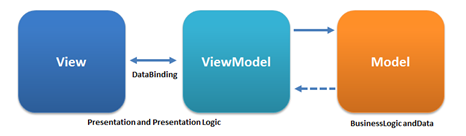
\includegraphics[width=12cm]{mvvm.png}
\caption{MVVM Schema}
\label{mvvm}

\end{center}
\end{figure}

Vue.js verbindet die sichtbaren Elemente und die Datensicht eines Systems selbstst"andig. Damit reagiert es automatisch bei "Anderung von Variablen und  stellt diese mittels DOM-Manipulationen und Output Formatting dar.\\

Das Herzst"uck der Vue.js-Bibliothek sind jedoch die Komponenten, mit denen sich komplexe Strukturen abbilden lassen. Wie bei anderen Systemen k"onnen sie weitere Komponenten enthalten.\\
Die Parent-Komponenten bestimmen dabei die Eigenschaften der Child-Komponenten. Die Kommunikation zwischen den Komponenten untereinander wird mit einem Event-System realisiert.\\

Au"serdem bietet Vue.js M"oglichkeiten beim Ein"ugen von neuen Elementen, diese mit animierten Effekten oder "Uberg"angen zu versch"onern.\\

Bei der Erstellung der Webapplikation Appcimo sorgen vor allem \textbf{Direktiven} f"ur "ubersichtliche und leicht-verst"andliche Code-Abschnitte. Damit lassen sich zum Beispiel Schleifen durch ein Array iterieren, HTML-Knoten optional einbinden (v-if) und ausblenden (v-show), Klickevents abfangen (v-on) und Attribute an Variablen binden (v-bind).


\section{Node.js und NPM}
Appcimo wird mit Hilfe der open-source JavaScript Runtime \textbf{Node.JS} erstellt. Es wird von der \textbf{Node.js Foundation} entwickelt und vertrieben. \\

\begin{figure} [h]
\begin{center}



\includegraphics[width=8cm]{nodejs.png}
\caption{Node.JS Logo}
\label{nodejs}

\end{center}
\end{figure}

Node.JS wird ben"otigt, um dem Javascript-Programm eine Laufzeitumgebung zur Verf"ugung zu stellen und den Quellcode mittels des Node.JS Interpreters einzulesen, zu analysieren und auszuf"uhren. Dadurch kann Javascript-Code auf einem Server lauff"ahig gemacht werden.\\

Die aktuelle Node.JS Version kann auf der offiziellen Seite https://nodejs.org/en/ gratis heruntergeladen und installiert werden.\\

Mit der Installation von Node.JS wird auch der \textbf{Node.JS Package Manager} zur Verf"ugung gestellt.\\

\begin{figure} [h]
\begin{center}



\includegraphics[width=8cm]{npm.png}
\caption{Node.JS Package Manager Logo}
\label{npm}

\end{center}
\end{figure}


Der npm Package Manager ist eine Platform f"ur Javascript-Entwickler, die Ihren Code oder Teile Ihres Codes f"ur andere Entwickler zur Verf"ugung stellen m"ochten. Dieser Code wird in Packages oder Module geb"undelt, die JavaScript-Bibliotheken enthalten. Ein Package ist ein Verzeichnis, das eine oder mehrere Dateien enth"alt. In ihnen gibt es typischerweise die Datei \textbf{package.json}, die einige Meta-Daten zu dem Package enth"alt. \\

Packages sind relativ klein und meistens nur f"ur einen bestimmten Zweck gedacht. Die Idee hier ist, mittels mehrerer kleiner  Packages ma"sgeschneiderte L"osungen f"ur die eigene Applikation zu konstruieren. \\

Die Packages und Module werden "uber die offizielle npm Seite www.npmjs.com/ zum Download angeboten. Sie werden "ublicherweise "uber den Bash/Cmd Konsolenbefehl npm install [...] installiert. Sie werden dann als Komponenten in die Applikation eingef"ugt und in dem Projekt-Verzeichnis \textbf{nodemodules} abgelegt.\\

Mittels des Package-Managers lassen sich die f"ur das eigene Programm verwendeten Packages leicht verwalten und auch updaten. \\


Durch die Verwendung des Webpack Templates werden eine Vielzahl an Tools und Modulen f"ur die Webseitenerstellung bereitgestellt. Neben dieser Grundinstallation wurden folgende npm Packages nachtr"aglich installiert:

\begin{figure} [H]
\begin{center}
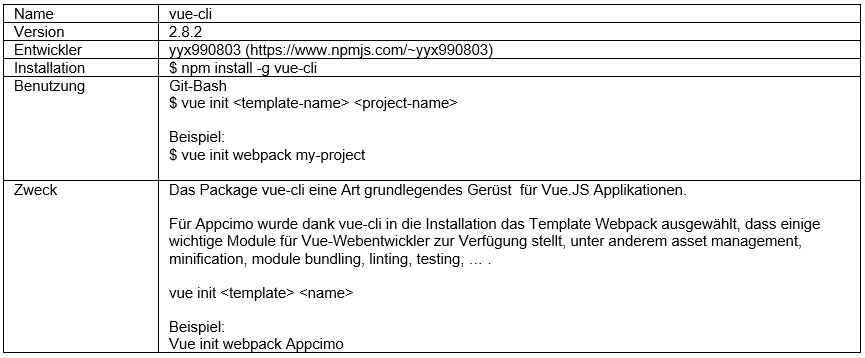
\includegraphics[scale=0.7]{package2.png}
\label{vue-cli}
\end{center}
\end{figure}



\begin{figure} [H]
\begin{center}
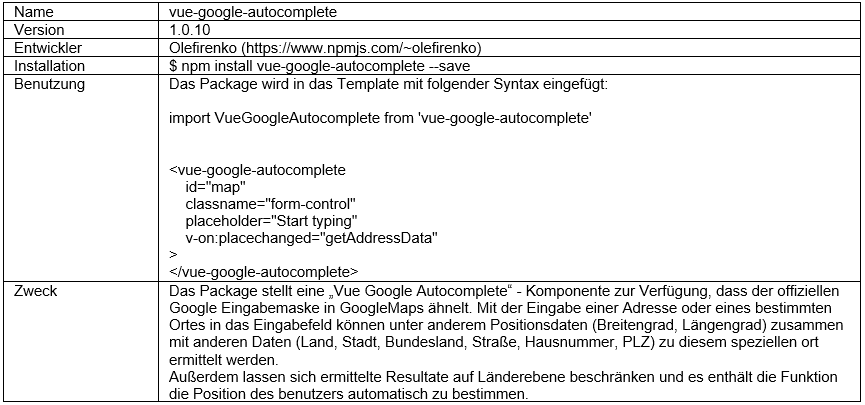
\includegraphics[scale=0.7]{package1.png}
\label{autocomplete}
\end{center}
\end{figure}


\begin{figure} [H]
\begin{center}
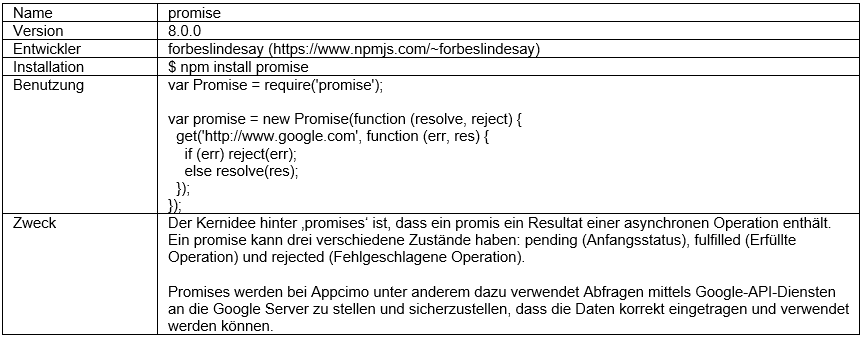
\includegraphics[scale=0.7]{package3.png}
\label{promise}
\end{center}
\end{figure}

\begin{figure} [H]
\begin{center}
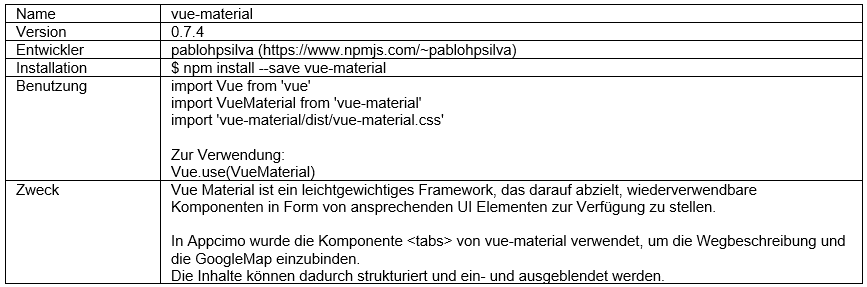
\includegraphics[scale=0.7]{package4.png}
\label{vue-material}
\end{center}
\end{figure}

\begin{figure} [H]
\begin{center}
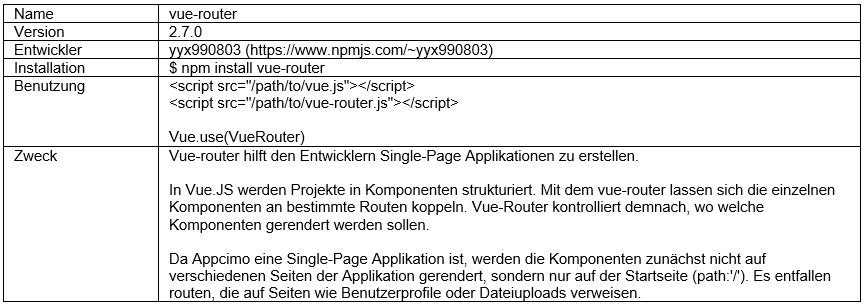
\includegraphics[scale=0.7]{package5.png}
\label{vue-router}
\end{center}
\end{figure}

\begin{figure} [H]
\begin{center}
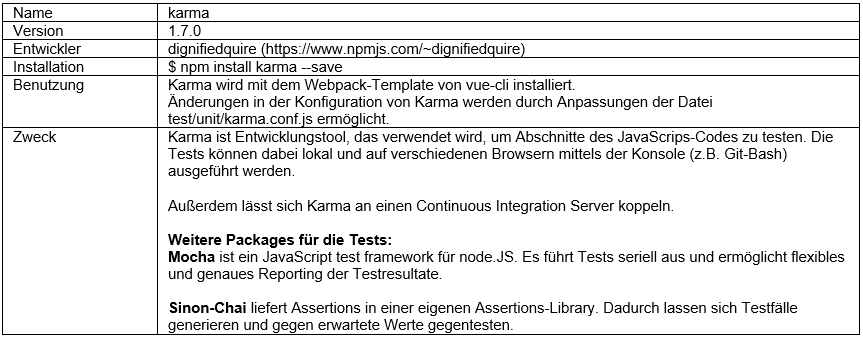
\includegraphics[scale=0.7]{package6.png}
\label{karma}
\end{center}
\end{figure}




\section{Github}
Appcimo wird mit dem Verison Control System \textbf{Git} auf \textbf{Github} gespeichert.
Dadurch wird eine transparente und sichere Erstellung der Applikation gew"ahrleistet. \\

\begin{figure} [H]
\begin{center}

\includegraphics[scale=0.7]{github.png}
\caption{GitHub Logo}
\label{github}
\end{center}
\end{figure}

https://github.com/Patida/acm \\

Hierf"ur wurden Entwickler des Teams als Contributer f"ur das Projekt freigeschaltet. \\

\textbf{Git-Hub Accounts} \\
https://github.com/schwetim \\
https://github.com/ARCMereel \\
https://github.com/PattnOne \\


Das \textbf{Repository} enth"alt den gesamten Code des Projekts, zuz"uglich der Tests und der Dokumentation und wird an einem Master Branch erstellt. \\
"anderungen an dem Programm-Code werden von den Projektmitgliedern commitet und gepusht, so dass alle Entwickler dauerhaft Zugriff auf die aktuellste Programm-Version haben. \\

Durch Kommentare bei jedem Commit, kennen alle Entwickler den aktuellen Stand und die Gr"unde des Pushs.  \\
Bei Push-"Uberschneidungen werden die Branches gemerged, so dass alle "Anderungen und Features im neuen Versionsstand enthalten sind. \\


\section{CircleCI}
\textbf{CircleCI} ist eine Continuous Integration und Release Platform. \\

\begin{figure} [H]
\begin{center}

\includegraphics[scale=0.7]{circle.png}
\caption{CircleCI Logo}
\label{circleci}
\end{center}
\end{figure}

CircleCI automatisiert den Build-, Test-, und Deploy-Prozess von Applikationen.
Bei der Einrichtung des CircleCI accounts, wird das Github Repository "uber eine Schnittstelle mit CircleCI verkn"upft. \\
Somit kann CircleCI auf den kompletten Code zugreifen und Tools und Services zur Verf"ugung stellen. \\

Der Software-Build kann "uber ein modernes UI gesteuert und beobachtet werden. \\

\begin{figure} [H]
\begin{center}
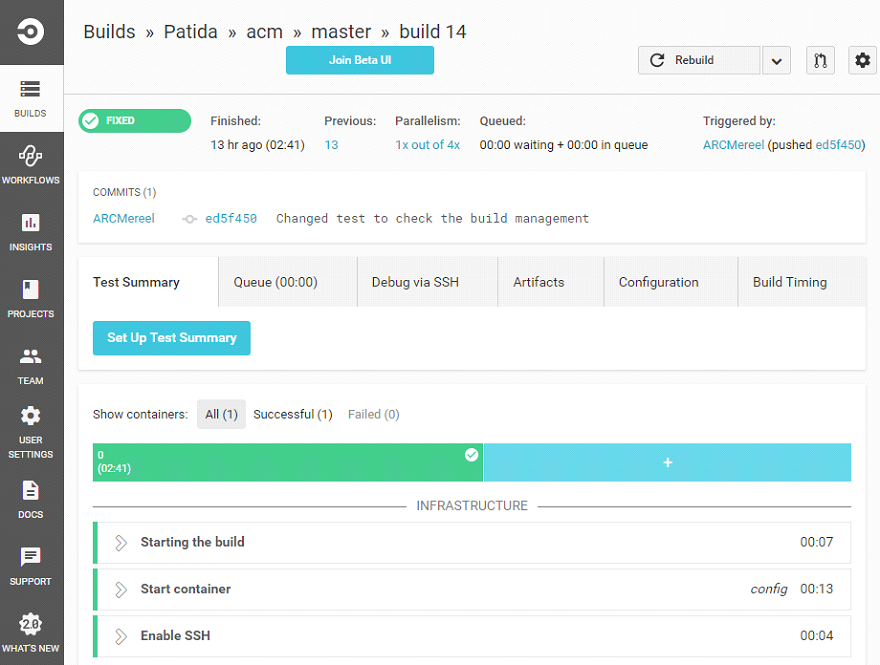
\includegraphics[scale=0.7]{build1.png}
\caption{CircleCI Starteseite}
\label{circleci}
\end{center}
\end{figure}

Da der Software-Build inklusive aller Tests logisch ausgef"uhrt wird, kann auf das Konsolen-Reporting der Testf"alle innerhalb der CircleCI UI zugegriffen werden. \\


\begin{figure} [H]
\begin{center}
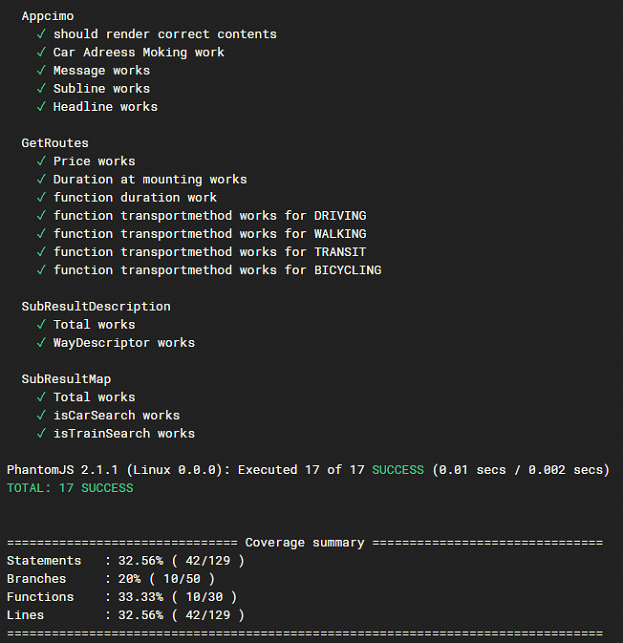
\includegraphics[scale=0.7]{build2.png}
\caption{Ausschnitt der Appcimo-Testauswertung}
\label{circlecitest}
\end{center}
\end{figure}


\textbf{AWS S3} \\
Ein weiteres Feature von CircleCI ist die Koppelung des CircleCI-Accounts mit einem Amazon AWS Account. \\
"Uber eine Schnittstelle zu Amazons Web Services ist CircleCI in der Lage, nach erfolgreichem Test, die Applikation oder den Build der Applikation zu einem Amazon AWS S3 Speicherort hochzuladen (deployen).\\

\begin{figure} [H]
\begin{center}
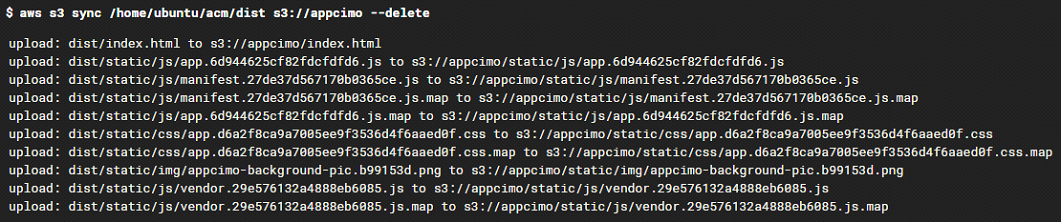
\includegraphics[scale=0.7]{build3.png}
\caption{Application Build - CircleCI}
\label{circlecitest}
\end{center}
\end{figure}



\textbf{Link zur Applikation: } http://appcimo.s3-website-eu-west-1.amazonaws.com/


\section{Google Services}

F"ur die Einbindung von Google-Services wie die Ermittlung von Positionsdaten, GoogleMaps und Routenberechnungen wird die Einbindung einer Google-API mit g"ultigem Key in die Applikation vorausgesetzt. \\

Die Beantragung eines Keys erfolgt "uber den Google API Manager. Voraussetzung hierf"ur ist ein Google-Konto.\\

Folgende Google-Services werden f"ur Appcimo ben"otigt.

\begin{figure} [H]
\begin{center}
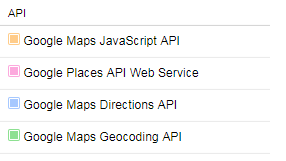
\includegraphics[scale=1]{google1.png}
\caption{Google API's}
\label{googleapi}
\end{center}
\end{figure}

Google stellt daf"ur ein Tageskontingent von 1.000 kostenlosen Anfragen an die Places Library pro Tag zur Verf"ugung.\\
Die "Uberwachung der API-Nutzung, eventuelle Latenzen und "Ubertragungsfehler lassen sich auch im Google-API Dashboard aufrufen.

\begin{figure} [H]
\begin{center}
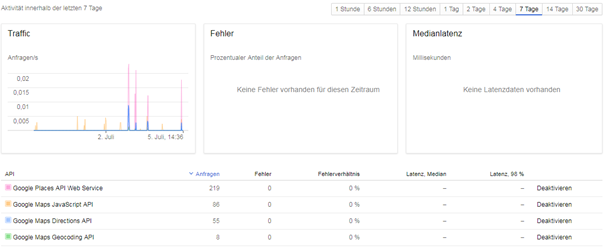
\includegraphics[scale=1]{google2.png}
\caption{Google API Dashboard}
\label{googledashboard}
\end{center}
\end{figure}


\chapter{Systementwurf und Umsetzung}

\section{Architektur}

\subsection{Systemarchitektur}
Die Entwicklung der Webapplikation richtet sich entsprechend VueJS nach der MVVM Model-View-ViewModel Architektur. \\
Um diese simple Architektur auf die Applikation anzuwenden, wird das Komponentendiagramm abstrakt genutzt. Das folgende Diagramm veranschaulicht, dass das View- und Viewmodell-Layer in der VueJS-Applikation selbst zu finden ist. In den einzelnen Vue-Komponenten sind sowohl die View, als auch die Steuerung und die Business Logic implementiert. \\

Das Backend/ Modell wird hierbei durch die Google-API und die Car2go-API (Car2go-API wird momentan nur simuliert) abgebildet. In ihnen werden die Routenberechnungen durchgef"uhrt und an das ViewModell zur"uckgegeben. Im ViewModell werden diese Routen dann weiter f"ur die View aufgearbeitet.\\

\begin{figure} [H]
\begin{center}
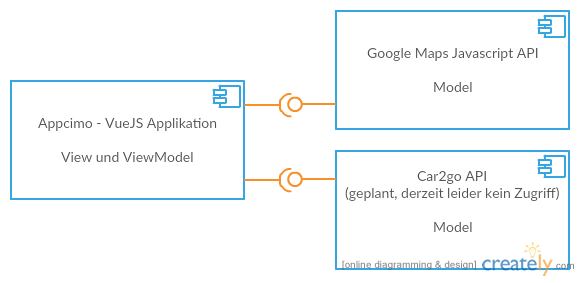
\includegraphics[scale=1]{mvvmappcimo.png}
\caption{MVVM Appcimo}
\label{MVVMAppcimo}
\end{center}
\end{figure}

\subsection{Komponentendiagramm}
Im Komponentendiagramm sind die einzelnen Vue-Komponenten sowie ihre Zugriffe untereinander abgebildet. Das Interface der Komponente stellen hierbei die „Properties“ von diesen dar. Durch Properties, und nur durch diese, k"onnen Daten in der Applikation von einer Komponente zur n"achsten gereicht werden.


\begin{figure} [H]
\begin{center}
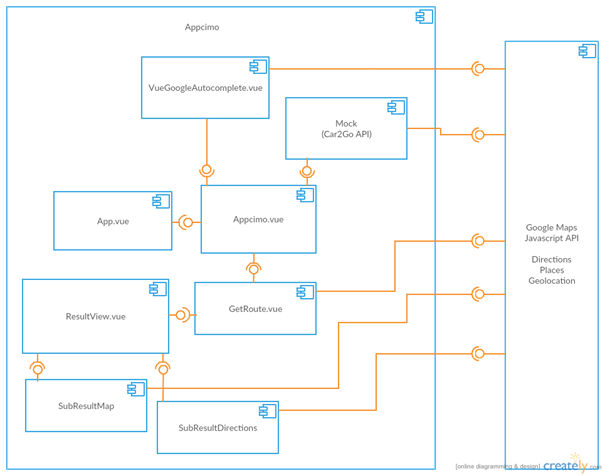
\includegraphics[scale=1]{komponentendiagramm.png}
\caption{Komponentendiagramm}
\label{Komponentendiagramm}
\end{center}
\end{figure}


\subsection{Komponentenbeschreibung}
Komponenten sind eines der m"achtigsten Features in Vue. Durch sie ist es m"oglich, HTML-Elemente und die damit verbundenen Sctipt- und Style-Elemente wiederverwendbar zu machen.  Diese Komponenten k"onnen auf das Nutzerverhalten oder Events reagieren und Werte und  Attribute aktiv modifizieren und bereitstellen.\\

\textbf{Komponenten} \\

\textbf{1. Appcimo.vue} \\

\textbf{Appcimo.vue} ist die Hauptkomponente der Webapplikation.  Alle weiteren Komponenten sind entweder in die Appcimo-Komponente eingesetzt oder in Unterkomponenten von Appcimo.vue eingesetzt.\\



\begin{figure} [H]
\begin{center}
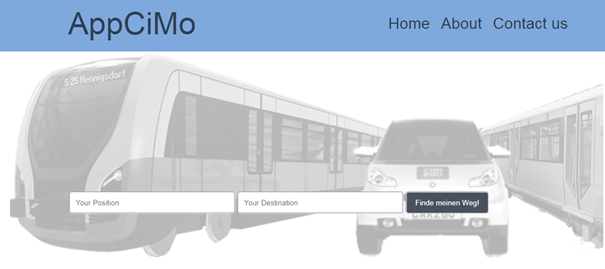
\includegraphics[scale=1]{compAppcimo.png}
\caption{Komponente Appcimo.vue}
\label{Appcimo}
\end{center}
\end{figure}

Appcimo.vue enth"alt die grunds"atzlichen Style-Elemente f"ur das Logo der Seite, die Top-Navigation, den Hintergrund und die einzelnen Untermen"us. Au"serdem enth"alt diese Komponente den Button, der die Methode getRoutes() startet: Finde meinen Weg!\\

\textbf{Enthaltene Komponenten:} VueGoogleAutocomplete, GetRoutes. \\

\textbf{Funktionen} \\

\textbf{getOrigin()}: Ermittelt durch Auswertung der VueGoogleAutocomplete-Komponente die Geoinformationen vom Startpunkt und "uber die GoogleMaps-API den n"achstgelegenen Car2Go Standort. \\

\textbf{getDestination()}:  Ermittelt durch Auswertung der VueGoogleAutocomplete-Komponente die Geoinformationen vom Zielort.\\

\textbf{getRoutes()}: Startet den Prozess die Komponente GetRoutes.vue zu rendern und sichtbar zu machen.\\

\textbf{mockCarAddress()}: Simuliert zu Testzwecken einen Standort eines Car2Go-Autos.\\

\textbf{getCarLocation()}: Ermittelt "uber den asynchronen Google geocode service den Standort des n"achstgelegenen Car2Go-Autos als ein Google geocode Objekt.\\


\textbf{2. VueGoogleAutocomplete.vue}

\begin{figure} [H]
\begin{center}
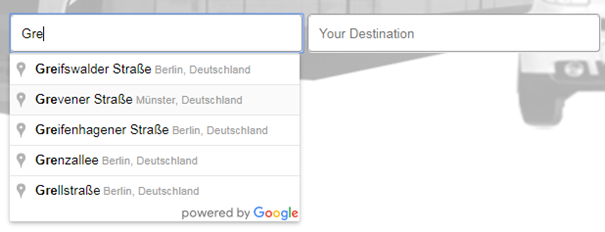
\includegraphics[scale=1]{autocomplete.png}
\caption{Komponente VueGoogleAutocomplete.vue}
\label{Autocomplete}
\end{center}
\end{figure}

\textbf{VueGoogleAutocomplete} wurde "uber den npm-Manager installiert. Diese Komponente stellt eine Inputbox, entsprechende Styleelemente und Google-API-Funktionalit"aten zur Verf"ugung. Durch diese Komponente k"onnen beliebige Adressen den entsprechenden Geoinformationen (Breitengrad, L"angengrad) zugeordnet werden.\\

Es werden zwei VueGoogleAutocomplete-Komponenten verwendet. Eine f"ur den Startpunkt, bzw. den aktuellen Standort und eine Komponente f"ur den Zielort bzw. die Zieladresse. Die ermittelten Geoinformationen werden in den entsprechenden Properties von Appcimo.vue zwischengespeichert.\\


\textbf{3. GetRoutes.vue}\\

\textbf{GetRoutes.vue} enth"alt die Business-Logic des Programms. \\

\textbf{Enthaltene Komponenten}: ResultView\\

\textbf{Funktionen:}\\

\textbf{getRoutes()}: Ermittlung und Speicherung der zur Auswahl stehenden Transportm"oglichkeiten mittels Promise-Funktionen. Die Promise-Funktionen dienen dabei als Zusicherung eines zur"uckerhaltenen Wertes durch die Google-API Calls. \\

\textbf{GetRoute()}:  Gibt alle Promise-Resultate der Funktionen wieder, die den Parameter "promises" enthalten. Diese Funktion wird ben"otigt, um mehrere zeitgleiche asynchrone google javascript api Calls auszuwerten. Dadurch „wartet“ die getRoutes-Funktion auf Ergebnisse, bevor die Berechnungen der erhaltenen Werte starten k"onnen.\\

\textbf{GoogleRouteQuery()}: Erm"oglicht asynchrone Benutzung der Google Javascript API, um Routen zu ermitteln. Diese Funktion gibt ein „Promise“ zur"uck, das den Empfang von Werten durch API Calls signalisiert.\\

\textbf{getShortinfo()}:  Berechnet die Werte, die in der Shortview ausgegeben werden. Dies beinhaltet die Startzeit  und die Ankunftszeit f"ur jede der Transportm"oglichkeiten. Diese Werte werden in Form eines JSON-Objekts zur"uckgegeben. \\

\textbf{getDescription()}: Gibt die Google-Ergebnisse der SubResultDescription wieder, um Wegbeschreibungen auf der Seiten anzeigen zu k"onnen. Au"serdem werden Ergebnisse f"ur den Fu"sweg anhand der Wegpunkte aussortiert, da diese falsch sein w"urden.\\

\textbf{getMap()}: "uber Sortiermechanismen werden die Ergebnisse des Google-API Calls gefiltert und zur Speicherung wiedergegeben.\\

\textbf{transportmethod()}:  Formatiert die Transportmethode und gibt sie zur"uck.

\begin{figure} [H]
\begin{center}
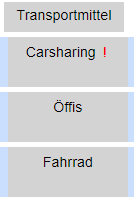
\includegraphics[scale=1]{transportmethod.png}
\caption{Transportmethod in Appcimo}
\label{transportmethod}
\end{center}
\end{figure}


\textbf{duration()}:  Die Fahrtdauer wird addiert, um ein Endergebnis f"ur die Dauer zu erhalten. F"ur CarSharing-Transportmethoden werden 4 Minuten zus"atzlich berechnet.


\begin{figure} [H]
\begin{center}
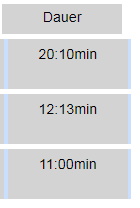
\includegraphics[scale=1]{duration.png}
\caption{Duration in Appcimo}
\label{Duration}
\end{center}
\end{figure}


\textbf{end()}:  Berechnung der Ankunftszeit. Diese Funktion wird nur f"ur CarSharing-Angebote ben"otigt.  Es werden 4 Minuten zus"atzlich berechnet.

\begin{figure} [H]
\begin{center}
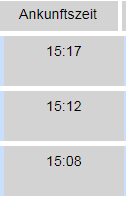
\includegraphics[scale=1]{end.png}
\caption{Ankunftszeit in Appcimo}
\label{end}
\end{center}
\end{figure}

\textbf{price()}:  Berechnung des Preises f"ur den Transport. Der Preis f"ur die "offentlichen Verkehrsmittel ist momentan noch fix.

\begin{figure} [H]
\begin{center}
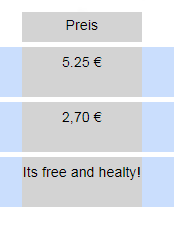
\includegraphics[scale=1]{price.png}
\caption{Preisberechnung in Appcimo}
\label{price}
\end{center}
\end{figure}

\textbf{4. ResultView.vue}\\

Die Komponente \textbf{ResultView.vue} stellt eine Zusammenfassung der ermittelten Transportm"oglichkeiten in Form von ausklappbaren Leisten dar. \\

\begin{figure} [H]
\begin{center}
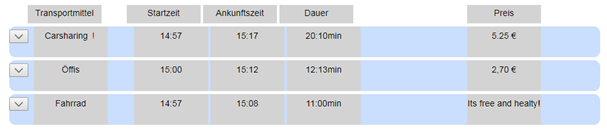
\includegraphics[scale=1]{resultview.png}
\caption{Komponente ResultView.vue}
\label{resultview}
\end{center}
\end{figure}

Die Ergebnisleisten werden bei einem Klick mittels eines Transition-Effekts ausgeklappt und die Details zur jeweiligen Transportm"oglichkeit abgerufen und ausgegeben. Diese Komponente enth"alt eine Watcher-Funktionalit"at, um bei mehrmaliger Benutzung der Routenermittlung stets die aktuellen Ergebnisse anzuzeigen. \\

Zum jetzigen Stand ist die CarSharing-Option nicht vollst"andig implementiert, so dass die Car2Go-Standorte simuliert werden. Ein entsprechender Hinweis wird auf der Webseite abgebildet.\\

\textbf{Enthaltene Komponenten}: SubResultMap, SubResultDescription\\

\textbf{5. SubResultDescription.vue}\\

Diese Komponente enth"alt die Wegbeschreibung einer Route vom Startpunkt bis zum Zielpunkt.\\


\begin{figure} [H]
\begin{center}
\includegraphics[scale=1]{SubResultDescription.png}
\caption{Komponente SubResultDescription.vue}
\label{SubResultDescription}
\end{center}
\end{figure}

\textbf{Funktionen:}\\

\textbf{updateDescription()}: Ermittelt "uber einen API-Call an den Google-Direction-Service die Wegbeschreibung einer angefragten Route und rendert diese innerhalb der Komponente. Diese Funktion wird ausgef"uhrt, sobald die Komponente aufgerufen wird.\\

\textbf{6. SubResultMap.vue}\\

Die GoogleMap wird in dieser Komponente dargestellt.\\


\begin{figure} [H]
\begin{center}
\includegraphics[scale=1]{SubResultMap.png}
\caption{Komponente SubResultMap.vue}
\label{SubResultMap}
\end{center}
\end{figure}


\textbf{Funktionen:}\\

\textbf{initMap()}: Die GoogleMap wird beim Start der Komponente gerendert und anhand von vorher festgelegten Parametern (Zoom-Level der Karte, Initialstandort, ziehbare Karte)  dargestellt. Die direkte Einbindung des directionDisplay erm"oglicht es, die Route anhand von farbigen Pfaden und Wegpunkten darzustellen.\\


\subsection{Sequenzdiagramm}
Das Sequenzdiagramm stellt einen einfachen schematischen Ablauf der Routensuche dar. Die Funktionen sind nicht deckungsgleich zu den Funktionen der Komponenten benannt, da diese teils sehr verschachtelt sind und nicht zum einfachen Verst"andnis des Prozesses beitragen w"urden.\\

Vielmehr k"onnen die hier verwendeten Funktionsnamen als Funktionsbox gesehen werden, die alle Javascript-Funktionen beinhalten, die zur Realisierung des beabsichtigten R"uckgabewertes dienen.

\begin{figure} [H]
\begin{center}
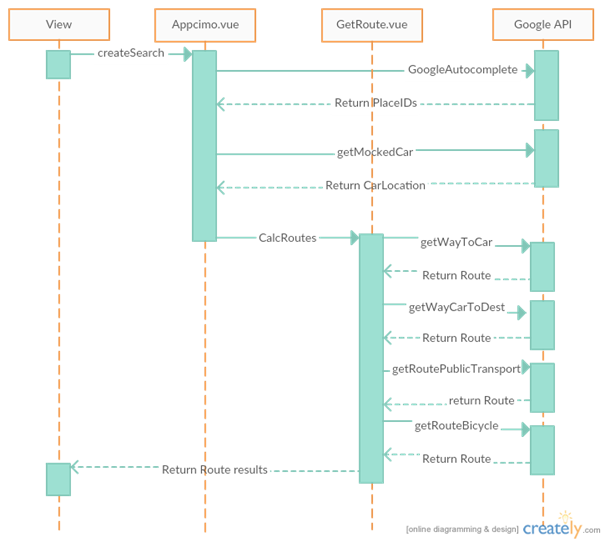
\includegraphics[scale=1]{sequenzdiagramm.png}
\caption{Sequenzdiagramm}
\label{Sequenzdiagramm}
\end{center}
\end{figure}

\section{Qualit"atsmanagement}

\subsection{Refactoring}
Um einen wartbaren Code zu schaffen, wurde regelm"a"sig ein Code-Refactoring betrieben.
Als Beispiel dient hier der erste Prototyp. Er funktionierte als Feldtest, war aber nur sehr schwer testbar und deshalb qualitativ nicht gut genug. Daraufhin wurden zwei gro"se Refactoring-Iterationen durchgef"uhrt, um wart- und testbaren Code zu erhalten.


\subsection{Unit Tests}
Unit-Tests sind bei dem Programm ein wichtiger Bestandteil um die gew"unschten Kernfunktionen der Applikation zu erhalten. Ein Refactoring sollte hierbei die Business Logic des Programms nicht negativ beeintr"achtigen.\\

Deshalb wurden entsprechende Unit Tests f"ur die Kernfunktionen der Applikation implementiert.

\subsection{Build-Management}
VueJS Applikationen sind in ihrem Entwicklungszustand nicht im Browser lauff"ahig. Sie m"ussen einem Build-Prozess unterzogen werden, bei dem die Vue-Dateien in HTML-, CSS- und Javascript-Dateien "ubersetzt werden.\\

Dies wird bei der Applikation Appcimo durch NodeJS und den entsprechenden npm Skripten gel"ost. Der Build-Prozess wird in der Build-Konfigurationsdatei „build.js“ definiert. Diese basiert auf weiteren Konfigurationsdateien. \\
Der Aufruf des Build-Prozesses wird durch npm scripts ausgel"ost. Diese sind wiederum in einer Konfigurationsdatei „package.json“ definiert. Hier werden die St"arken des einheitlichen JSON-Format genutzt. Es ist durch seinen strukturierten Aufbau f"ur viele Applikationen gut nutzbar.\\

Die in der package.json hinterlegten Ziele starten z.B. die build.js-Datei und k"onnen auf eventuelle Abh"angigkeiten verweisen. So ist es zum Beispiel m"oglich, die unit tests als Pre-Build Prozess zu konfigurieren (wie man es als Dependencies aus z.B. Ant kennt). Hierbei wird der Build erst ausgef"uhrt wenn das Testskript eine positive R"uckmeldung gibt.

\subsection{Continuous Integration}
Das Prinzip der Continuous Integration steuert einen gro"sen Teil zur Qualit"at der Software bei. Hier wird das Online-Tool „CircleCI“ genutzt, da es in Github integrierbar ist und die Build-Konfigurationen aus den package.json Konfigurationsdateien auslesen kann.\\

Wenn ein git-push zu dem Github-Repository durchgef"uhrt wird, startet CircleCI den Continuous Integration Prozess.\\

Zun"achst wird die Build-Umgebung abh"angig der package.json Konfiguration-Datei hergestellt. Danach erfolgt der Test und Build der Software. Hier werden die definierten npm Skripte ausgef"uhrt. Im Fall von Appcimo wird zun"achst der Test und abh"angig davon der Build ausgef"uhrt. Sind der Test und der Build erfolgreich, wird der definierte Deploy Prozess zu Amazon S3 durchgef"uhrt. Ist der Test hingegen nicht erfolgreich werden die App-Owner dar"uber benachrichtigt und der fehlerhafte Code wird nicht zur Live-Umgebung "ubertragen.


\chapter{Zusammenfassung und Ausblick}
Mit Abschluss des Semester-Projektes „Appcimo“ f"ur das Modul Softwaretechnik-Projekt wurde ein funktionierender und stabil-laufende Prototyp entwickelt. Durch die erstellten Testf"alle wird die korrekte Ausf"uhrung der Applikation sichergestellt. Die Einbindung der Continuous Integration Platform CircleCI erm"oglicht das Ausf"uhren und "Uberwachen des Software-Builds inklusive der Tests und erm"oglicht, das Programm auf einem Amazon AWS Server zu hosten. Der Software-Prototyp enth"alt die zuvor im Team abgestimmten Features.\\
F"ur die Zukunft ist jedoch noch eine Weiterentwicklung des Programms geplant. Unter anderem sollen weitere Carsharing-Anbieter als Transportm"oglichkeit integriert werden. Auch die Routenanfrage der "offentlichen Verkehrsmittel soll erweitert werden, eine detaillierte Auswahl an Fahrzeugtypen anbieten k"onnen (Ubahn, Sbahn, Tram, Bus, Regionalbahn) und Preise exakt berechnen k"onnen. \\

Das Template der Wegbeschreibung wird momentan von Google gestellt. Da alle Informationen des Weges als Objekt geliefert werden, ist es jedoch m"oglich eine individuelle, stilistisch auf das Programm abgestimmte Wegbeschreibung zu erstellen. \\

Zur Positionsermittlung wird momentan die Startadresse abgefragt und ausgewertet. Es soll zuk"unftig - bei Einwilligung - eine automatische Standorterfassung erfolgen, die die Koordinaten der Person als Startadresse verwendet, um noch schneller, flexibler und genauer Routen abzufragen.\\

Der Grundstein f"ur eine sinnvolle und innovative Webapplikation ist gelegt. Mit den festgelegten Ma"snahmen f"ur die Zukunft soll die Applikation ein gro"ses Publikum ansprechen und den besten Service f"ur die Zielerreichung in Gro"sst"adten liefern.\\


\chapter{Anh"ange}

\begingroup
	\renewcommand*{\addvspace}[1]{}
	\phantomsection
	\addcontentsline{toc}{chapter}{\listfigurename}
	\listoffigures
	\newpage
	\phantomsection
	\addcontentsline{toc}{chapter}{\listtablename}
	\listoftables
\endgroup


\end{document}
